\chapter{Details}
\indent
    Details are listed in this chapter including 5 parts, 
    $n$-tuple network, TD(0) algorithm, TD-backup diagram, action selection, and implementation details.

\section{$n$-tuple network} 
\begin{enumerate}
	\item Isomorphic patterns are created in constructor of class \code{pattern} (See Listing \ref{pattern-constructor}). 
\begin{lstlisting}[language=C++, caption={C++ code of class \textcolor{blue}{pattern} constructor.}, label={pattern-constructor}]
for (int i = 0; i < 8; i++) {
	board idx = 0xfedcba9876543210ull;
	if (i >= 4) idx.mirror();
	idx.rotate(i);
	// Get indices of isomorphic patterns on the board.
	for (int t : p) {
		isomorphic[i].push_back(idx.at(t));
	}
}\end{lstlisting}
	\item Get index of an isomorphic pattern of the board. 
\begin{lstlisting}[language=C++, caption={C++ code of \textcolor{blue}{indexof} function of class \textcolor{blue}{pattern}.}, label={pattern-indexof}]
size_t indexof(const std::vector<int>& patt, const board& b) const {
	// TODO
	size_t idx = 0;
	for (size_t i = 0; i < patt.size(); i++)
		idx |= b.at(patt[i]) << (4 * i); // Shift left 16 bits.

	return idx;
}\end{lstlisting}
	\item Values of isomorphic patterns are sum up to represent the value of the board (See Listing \ref{pattern-estimate}). 
\begin{lstlisting}[language=C++, caption={C++ code of \textcolor{blue}{estimate} function of class \textcolor{blue}{pattern}.}, label={pattern-estimate}]
virtual float estimate(const board& b) const {
	// TODO
	// Sum up values of all isomorphic patterns.
	float sum_iso_patterns = 0;
	for (int i = 0; i < iso_last; i++) 
		sum_iso_patterns += weight[indexof(isomorphic[i], b)];

	return sum_iso_patterns;
}\end{lstlisting}
	\item Update isomorphic patterns with mean error, and then return the updated weight (See Listing \ref{pattern-update}). 
\begin{lstlisting}[language=C++, caption={C++ code of \textcolor{blue}{update} function of class \textcolor{blue}{pattern}.}, label={pattern-update}]
virtual float update(const board& b, float u) {
	// TODO
	// Update all isomorphic patterns with mean.
	float mean = u / iso_last;
	float sum_iso_patterns = 0;
	for (int i = 0; i < iso_last; i++) {
		size_t idx = indexof(isomorphic[i], b);
		weight[idx] += mean;
		sum_iso_patterns += weight[idx];
	}

	return sum_iso_patterns;
}\end{lstlisting}
\end{enumerate}

\pagebreak
\section{TD(0) algorithm}
\indent
	This algorithm, starting from second last move of the episode, 
	calculates error between before-state of the move $s$ and next move $s''$, then 
	updates before-state of $s$ with the error, and finally 
	calculates TD target with sum of reward of $s$ and updated weight of before-state of $s$. 
	Keep the TD target for next step, repeat steps above till the start of the episode 
	(See Figure \ref{td-0-algorithm} and Listing \ref{learning-update-episode}). 
\begin{figure}[H]
	\centering
	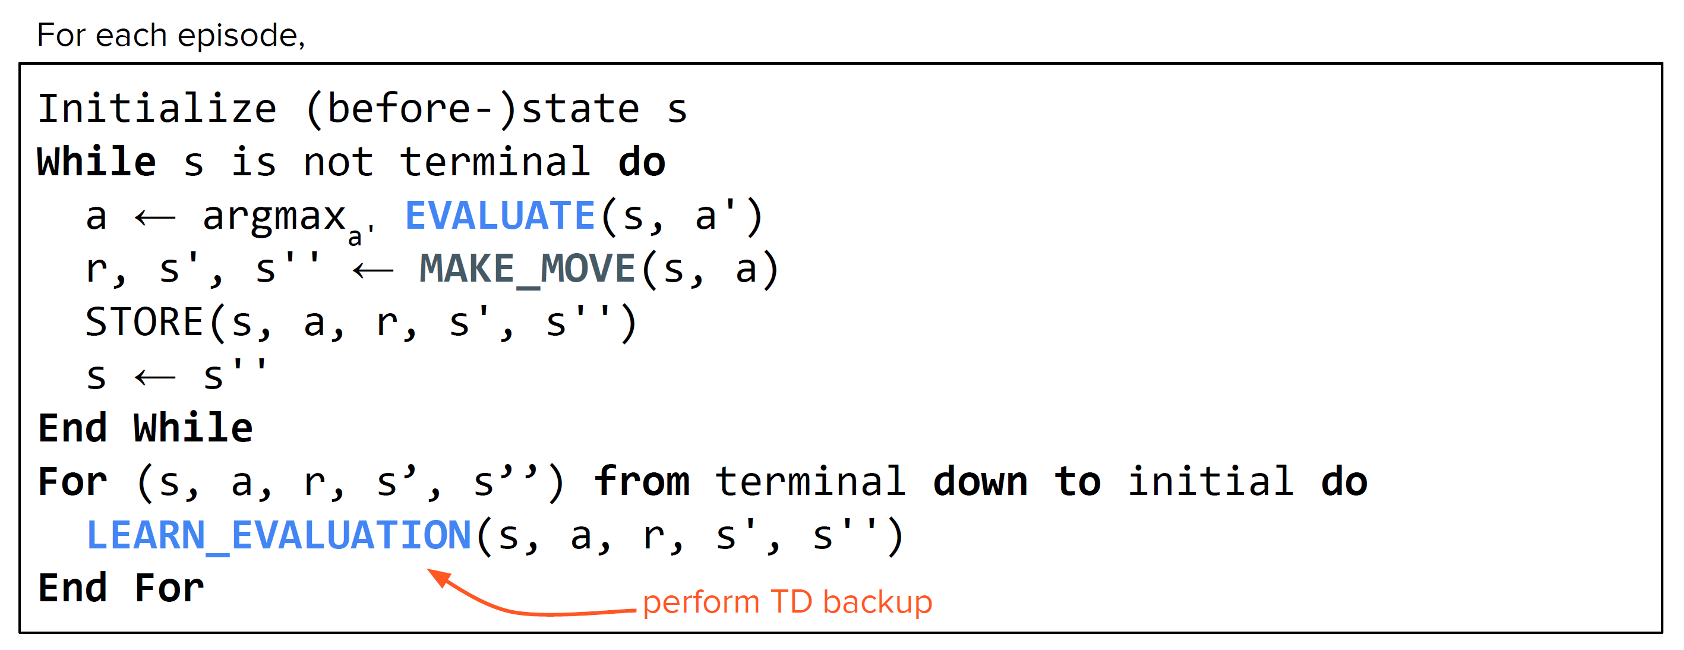
\includegraphics[scale=0.5]{img/td.png}
	\caption{Pseudo-code of TD(0) algorithm.}
	\label{td-0-algorithm}
\end{figure}
\begin{lstlisting}[language=C++, caption={C++ code of \textcolor{blue}{update\_episode} function of class \textcolor{blue}{learning}.}, label={learning-update-episode}]
void update_episode(std::vector<state>& path, float alpha = 0.1) const {
	// TODO
	// Starts from second last move, and update state backwards iteratively.
	float target = 0.0f;
	for (path.pop_back(); path.size(); path.pop_back()) {
		state& move = path.back();
		target = move.reward() + 
			update(move.before_state(), alpha * (target - (move.value() - move.reward())));
	}
}\end{lstlisting}

\pagebreak
\section{TD-backup diagram}
\begin{enumerate}
	\item Before-state: use before-state of move $s$ as value function, and use 
	reward $r$ and before-state of next move $s''$ as TD target to update before-state of the move $s$
	(See Figure \ref{td-backup-before-state}).
	\begin{figure}[H]
		\centering
		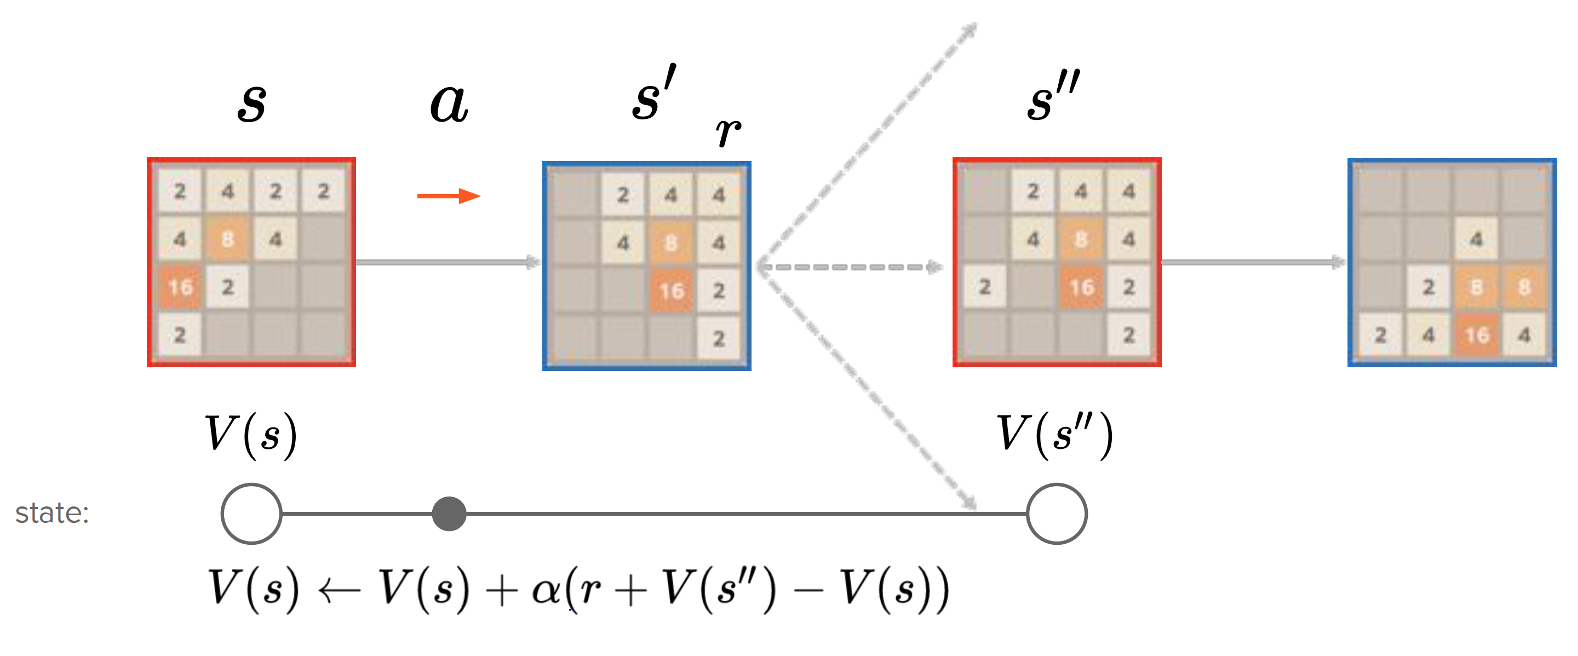
\includegraphics[scale=0.5]{img/td-backup-before-state.png}
		\caption{TD backup diagram of before-state.}
		\label{td-backup-before-state}
	\end{figure}
	\item After-state: use after-state of move $s'$ as value function, and use 
	reward $r_{next}$ and after-state of next move $s'_{next}$ as TD target to update after-state of the move $s'$
	(See Figure \ref{td-backup-after-state}).
	\begin{figure}[H]
		\centering
		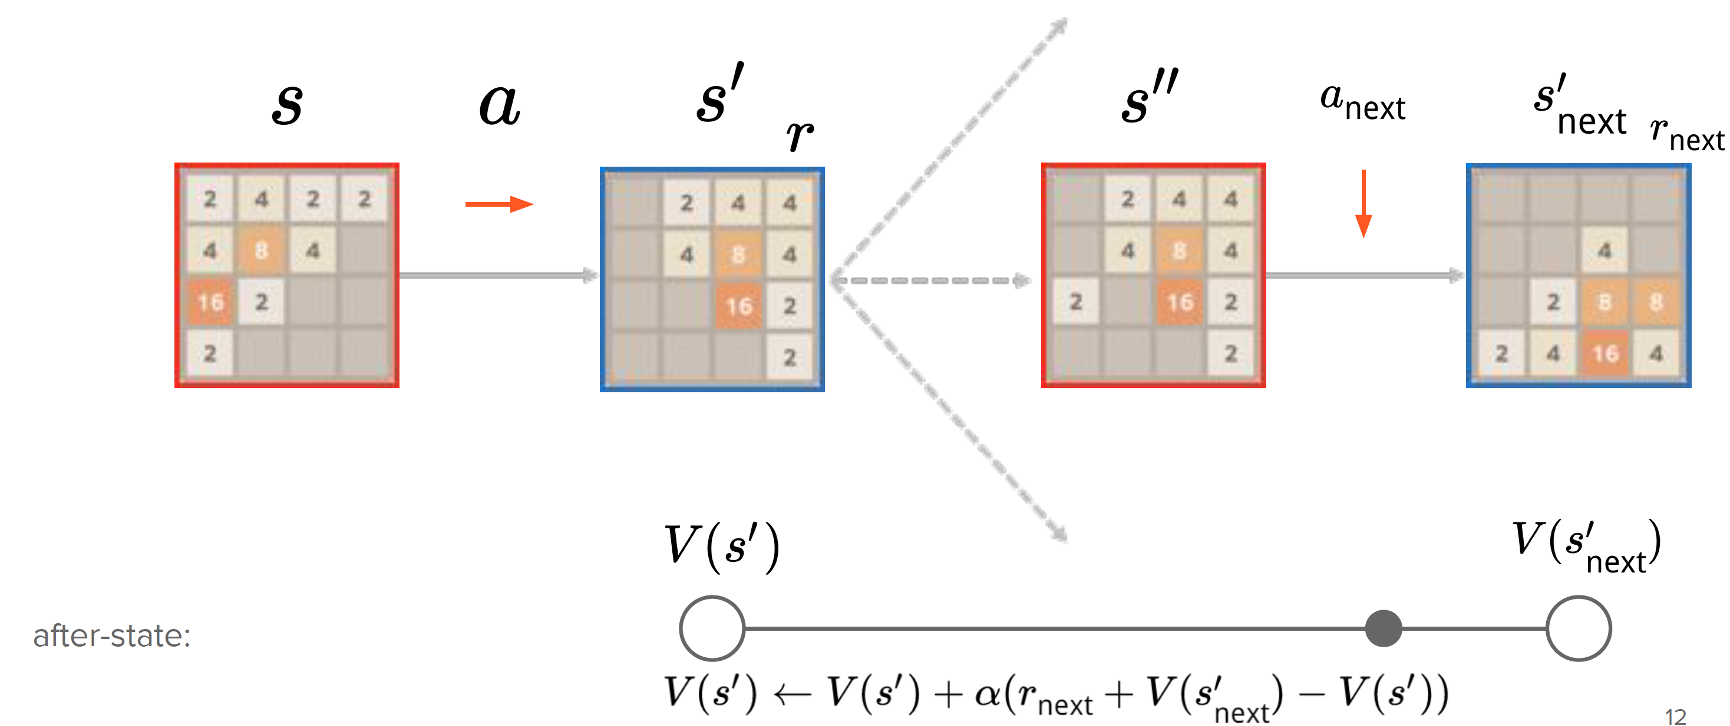
\includegraphics[scale=0.5]{img/td-backup-after-state.png}
		\caption{TD backup diagram of after-state.}
		\label{td-backup-after-state}
	\end{figure}
\end{enumerate}

\pagebreak
\section{Action selection}
\begin{enumerate}
	\item Before-state: after choosing an action $A_t$, randomly generate one 2-tile or 4-tile, then
	calculate and weighted sum up value functions of each new state $S_{t + 1}$ 
	by the probability that 2-tile and 4-tile pop-up and number of empty tiles
	(See Figure \ref{action-selection-before-state}).
	\begin{figure}[H]
		\centering
		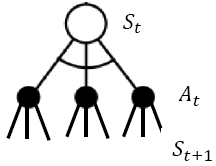
\includegraphics[scale=0.5]{img/action-selection-before-state.png}
		\caption{Action selection of before-state.}
		\label{action-selection-before-state}
	\end{figure}
	\item After-state: consider that before-state of next move $S_{t + 1}$ is fixed, and 
	when choosing action of next move $A_{t + 1}$ is the same situation, so this approach 
	chooses the action that results in highest value of after-state.
	(See Figure \ref{action-selection-after-state}).
	\begin{figure}[H]
		\centering
		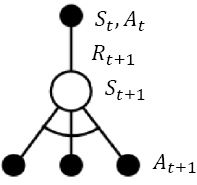
\includegraphics[scale=0.5]{img/action-selection-after-state.png}
		\caption{Action selection of after-state.}
		\label{action-selection-after-state}
	\end{figure}
\end{enumerate}

\section{Implementation details}
\begin{enumerate}
	\item \code{indexof} (See Listing \ref{pattern-indexof}), \code{estimate} (See Listing \ref{pattern-estimate}), 
	\code{update} (See Listing \ref{pattern-update}), \code{update_episode} (See Listing \ref{learning-update-episode}) functions have been listed in previous sections.
	\item First, find all empty tiles during after-state, then randomly generate 2-tile or 4-tile, and 
	calculate weighted sum to be the value of before-state of the move, and finally
	update the highest value for further comparisons, and return best move (See Listing \ref{learning-select-best-move}).
\begin{lstlisting}[language=C++, caption={C++ code of \textcolor{blue}{select\_best\_move} function of class \textcolor{blue}{learning}.}, label={learning-select-best-move}]
state select_best_move(const board& b) const {
	state after[4] = { 0, 1, 2, 3 }; // up, right, down, left
	float weight_2_tile = 0.9f;
	float weight_4_tile = 1.0f - weight_2_tile;

	state* best = after;
	float best_move_val = -std::numeric_limits<float>::max();
	for (state* move = after; move != after + 4; move++) {
		if (move->assign(b)) {
			// TODO
			board after_state = move->after_state();
			int tiles[16];
			int numEmptyTiles = 0;

			// Find all empty tiles during after-state.
			for (int i = 0; i < 16; i++)
				if (after_state.at(i) == 0)
					tiles[numEmptyTiles++] = i;

			// Find best move during after-state.
			float val = move->reward();
			for (int i = 0; i < numEmptyTiles; i++) {
				board* cur_board = new board(uint64_t(after_state));

				cur_board->set(tiles[i], 1); // 2-tile.
				val += weight_2_tile * (estimate(*cur_board) / numEmptyTiles);

				cur_board->set(tiles[i], 2); // 4-tile.
				val += weight_4_tile * (estimate(*cur_board) / numEmptyTiles);
			}
			
			move->set_value(estimate(move->before_state()));

			if (val > best_move_val) {
				best = move;
				best_move_val = val;
			}
		} else {
			move->set_value(-std::numeric_limits<float>::max());
		}
		debug << "test " << *move;
	}
	return *best;
}\end{lstlisting}
\pagebreak
	\item With original 4 patterns (See Listing \ref{patterns-original} and Figure \ref{patterns-org-illustration}), the average reached 2048-tile percentage is about \textcolor{blue}{\textbf{90\%}} after 350K iterations.
	However, with additional 4 patterns, totally 8 patterns (See Listing \ref{patterns-new} and Figure \ref{patterns-new-illustration}), it's about \textcolor{blue}{\textbf{95\%}} (Details are in Chapter \ref{chapter-results}).
\begin{lstlisting}[language=C++, caption={C++ code of original 4 patterns.}, label={patterns-original}]
tdl.add_feature(new pattern({ 0, 1, 2, 3, 4, 5 }));
tdl.add_feature(new pattern({ 4, 5, 6, 7, 8, 9 }));
tdl.add_feature(new pattern({ 0, 1, 2, 4, 5, 6 }));
tdl.add_feature(new pattern({ 4, 5, 6, 8, 9, 10 }));\end{lstlisting}
\begin{figure}[H]
	\centering
	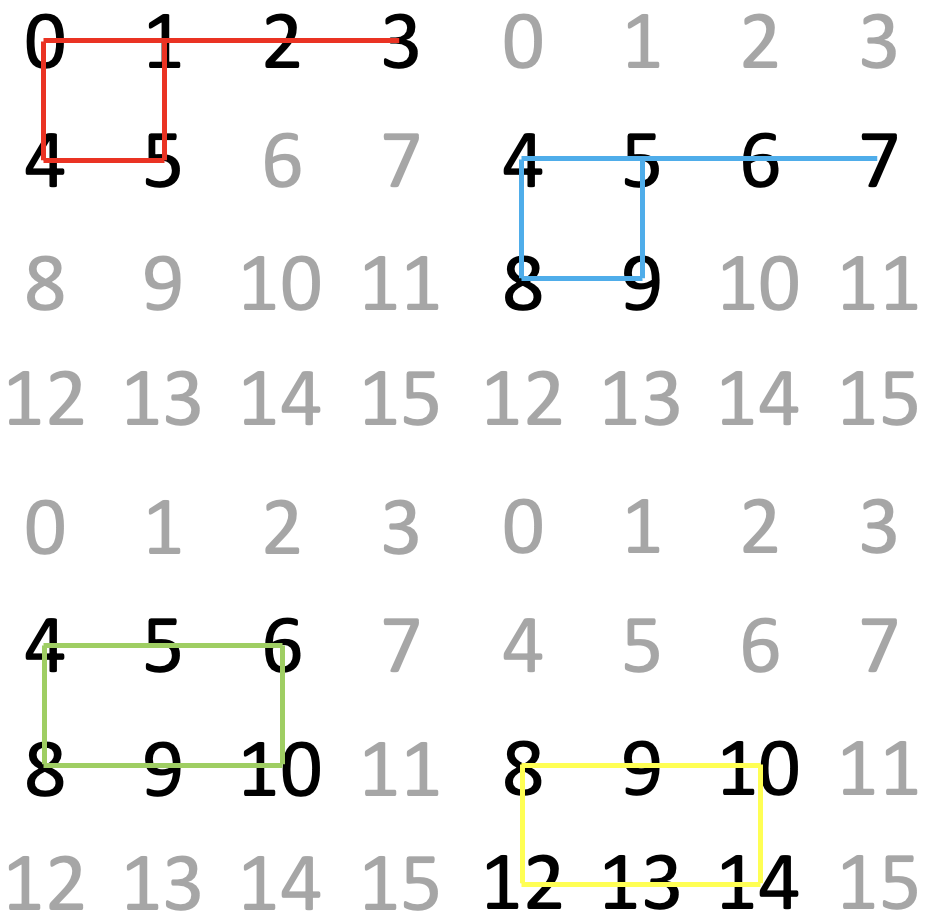
\includegraphics[scale=0.4]{img/patterns-org-illustration.png}
	\caption{Illustration of original 4 patterns.}
	\label{patterns-org-illustration}
\end{figure}
\begin{lstlisting}[language=C++, caption={C++ code of new 4 patterns.}, label={patterns-new}]
tdl.add_feature(new pattern({ 0, 2, 5, 10 }));
tdl.add_feature(new pattern({ 4, 6, 9, 14 }));
tdl.add_feature(new pattern({ 1, 4, 5, 6, 9, 13 }));
tdl.add_feature(new pattern({ 1, 4, 9, 14 }));\end{lstlisting}
\begin{figure}[H]
	\centering
	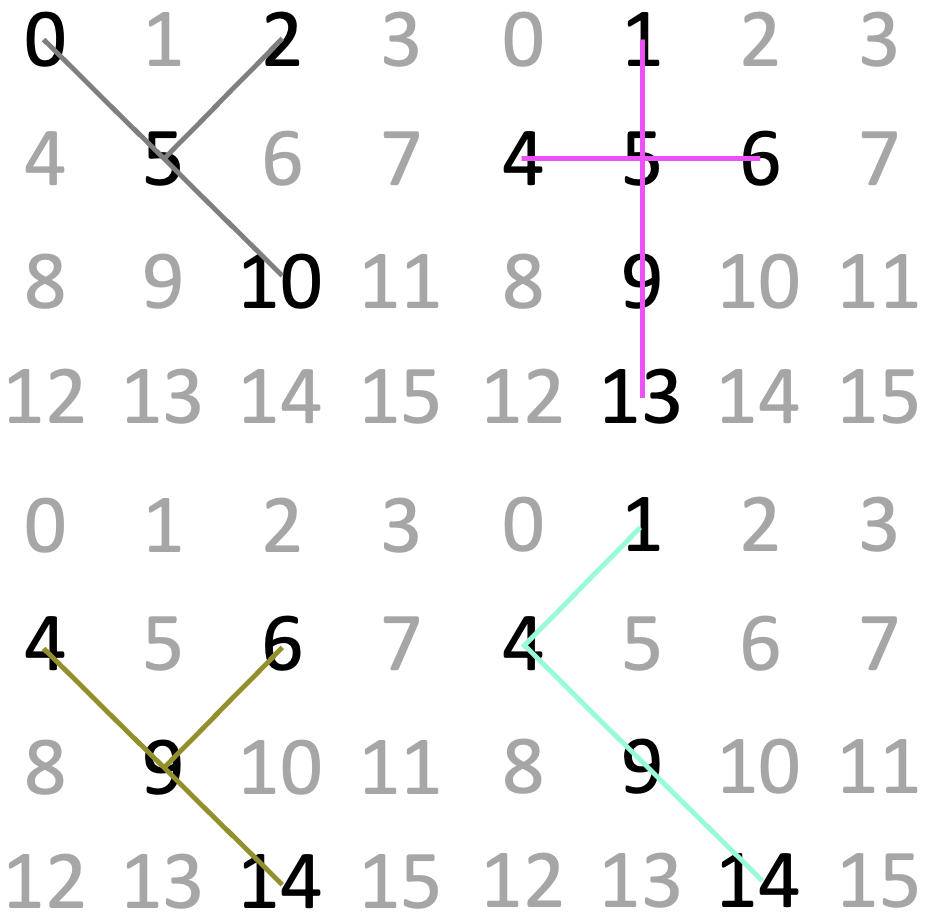
\includegraphics[scale=0.4]{img/patterns-new-illustration.png}
	\caption{Illustration of new 4 patterns.}
	\label{patterns-new-illustration}
\end{figure}
\end{enumerate}
